sainzsain\chapter{System-Design}
\label{cha:systemdesign}

\section{Architektur des dezentralen Identitätsmanagementsystems}

\subsection{Entscheidung über Framework}
Um sich für eine Architektur festzulegen, muss zunächst die Entscheidung über die darunterliegende Plattform getroffen werden. Dabei stehen die in Kapitel 5 betrachteten Lösungen zur Auswahl: Luniverse, Dock, PolygonId, Sovrin und Shocard. Für die Entwicklung des Prototypen wird im folgenden :
\begin{itemize}
	
	\item Polygon (als unterliegende Blockchain) zeigt folgende Vorteile auf \cite{ID54}:
	\begin{itemize}
		\item Die Blockchain skaliert hervorragend mit einer steigenden Anzahl von Transaktionen
		\item Geringe Transaktionskosten
		\item Hohe Interoperabilität mit Ethereum
		\item Etablierte Plattform und weite Verbreitung im Markt
	\end{itemize}
	
	\item PolygonId:
	\begin{itemize}
		\item Möglichkeit zum Widerruf von Informationen gegeben
		\item Informationen sind überprüfbar
		\item Selektive-Disclosure implementierbar
		\item Alle nicht-funktionalen Anforderungen implementierbar
		\item Unterstützt W3C Standard für VC's
		\item Credential Exchange erfolgt nach Identity-Foundation Standard
	\end{itemize}
\end{itemize}
Prinzipiell besteht die Architektur aus drei Komponenten: Einem Verifier, einem Issuer und dem Holder. Jede dieser drei Komponenten laufen unabhängig voneinander und können mit fremd-implementierten Instanzen kommunizieren. Das hier dargestellte Szenario ist das Erstellen, Übertragen und Verifizieren von einem digitalen Führerschein auf der Blockchain. Die System-Architektur sieht dabei wie folgt aus:
\begin{figure}[h]
	\centering
	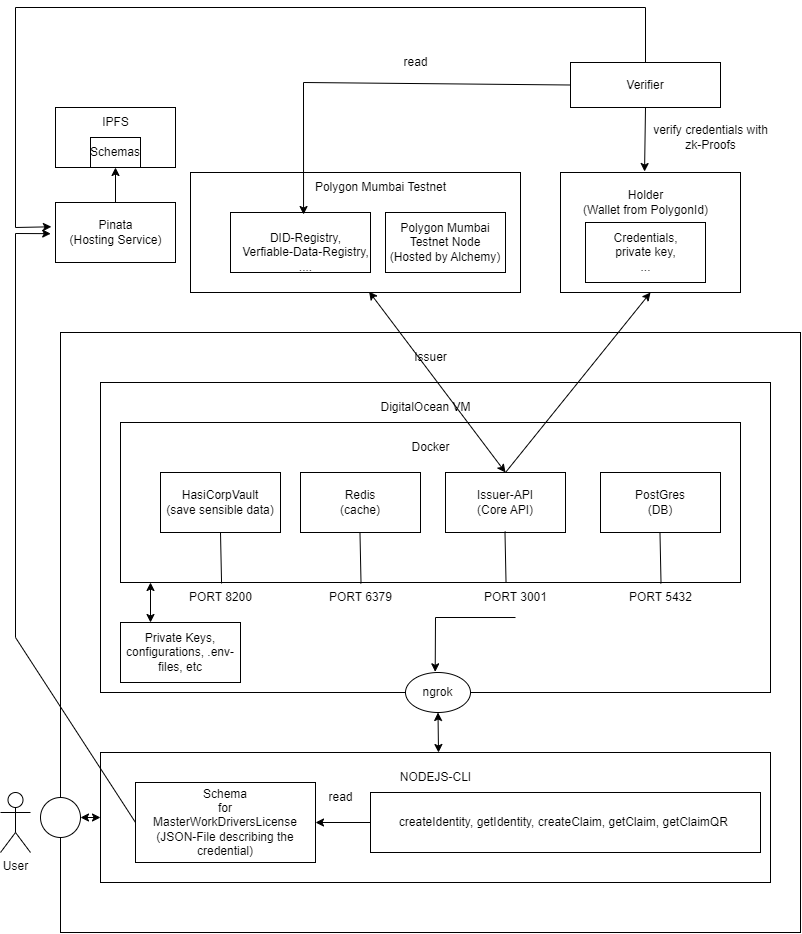
\includegraphics[scale=0.4]{media/system-design}
	\caption{System-Design des Prototyps}
	\label{fig:meine-grafik}
\end{figure}
Es ist zu erkennen, dass der Issuer die zentrale Komponente ist. Um den Issuer zu hosten wird eine virtuelle Maschine von DigitalOcean \footnote{https://www.digitalocean.com/} verwendet. VMs werden bei DigitalOcean auch Droplets genannt, wobei das Droplet für den Prototypen wie folgt konfiguriert ist:
\begin{figure}[h]
	\centering
	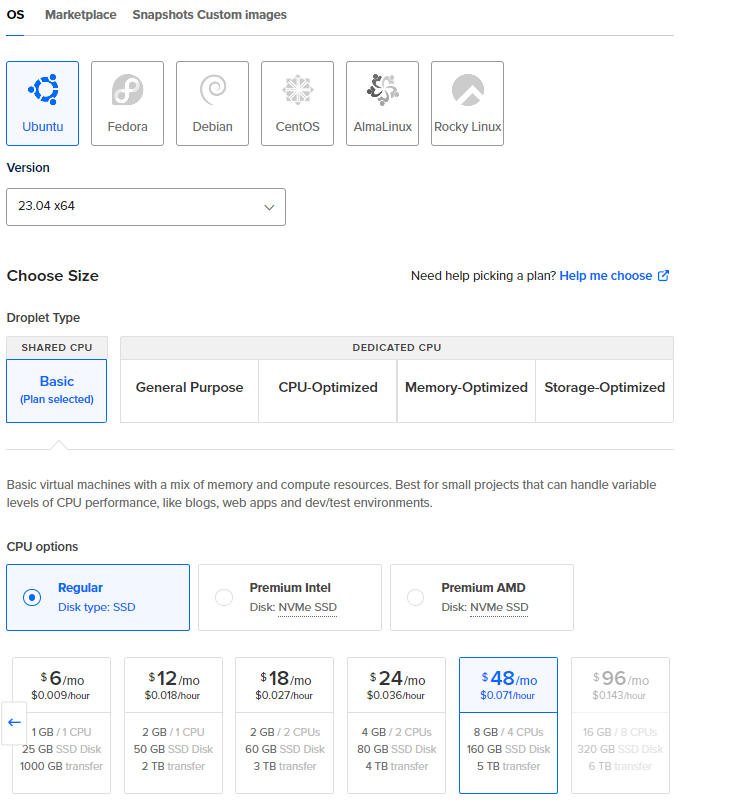
\includegraphics[scale=0.4]{media/config}
	\caption{Konfiguration des DigitalOcean-Droplets}
	\label{fig:meine-grafik}
\end{figure}
Auf dem Droplet läuft ein Docker der alle in der Grafik darstellen Container orchestriert. Der einzige Container, der auch von extern erreichbar sein muss ist der 'issuer-api'-Container, da er die REST-API Anfragen erhält. Für Letzteres wird 'ngrok' \footnote{https://ngrok.com/} verwendet, wobei ein Tunnel von einer öffentlichen IP auf den Lokalhost des Droplets gebaut wird. Dieser Tunnel wird vom NodeJs-Cli verwendet, um Anfragen über die API an den - von Alchemy \footnote{https://www.alchemy.com/} gehosteten - Netzwerk-Knoten weiterzuleiten. Die Schemas müssen öffentlich zugänglich sein, da sie unter anderem im Verifier und Issuer referenziert werden. Um dem ursprünglichen Gedanken der Dezentralität treu zu bleiben werden auch die Schemas dezentral - über IPFS \footnote{https://ipfs.tech/} - gespeichert. Als Schnittstelle zwischen IPFS und der Anwendung wird Pinata \footnote{https://www.pinata.cloud/} verwendet. Das dort gehostete Schema sieht hierbei wie folgt aus:
\begin{lstlisting}[language=json,firstnumber=1]	
		[...]
		"MasterWorkDriversLicense": {
			"@context": {
			 [...]
				"TypeOfVehicle": {
					"@id": "polygon-vocab:TypeOfVehicle",
					"@type": "xsd:string"
					[...]
					
					"enum": [
						"Car",
						"Truck",
						"Scooter",
						"Motorcycle"
					],
					
				},
				"YearOfReceipt": {
					"@id": "polygon-vocab:YearOfReceipt",
					"@type": "xsd:integer"
				}
			},
			[...]
		}
	}
	]
}
\end{lstlisting}
Es ist zu erkennen, dass der Führerschein für den Prototypen aus zwei Attributen besteht:
\begin{itemize}
	\item YearOfReceipt: Ein Integer, der das Jahr darstellt an dem der Holder den Führerschein erworben hat
	\item TypeOfVehicle: Ein String, der den Typ des Vehicle beschreibt. Hierbei gibt es vier Typen: 
	
	\begin{itemize}
		\item Car
		\item Truck
		\item Scooter
		\item Motorcycle
	\end{itemize}
\end{itemize}}]

Zum Erstellen der Schemata stellt PolygonId einen Schema-Builder zur Verfügung \footnote{https://schema-builder.polygonid.me/}. \\
Nachdem der Issuer den Führerschein ausgestellt hat kann der Holder ihn entgegennehmen. Der nächste Schritt ist, dass ein Verifier einen Query definiert, der wie folgt aussehen könnte:
\begin{lstlisting}[language=json,firstnumber=1]	
	id: 1,
	circuitId: 'credentialAtomicQuerySigV2', // algorithmus zum Erstellen des zk-Proofs
	query: {
		allowedIssuers: ['*'],
		type: 'MasterWorkDriversLicense', // im Schema definierter Typ
		context: 'https://ipfs.io/ipfs/QmTSd6saivXHysRopQdM1yswp2qyFwobL7fwuFpkVTS8gd', // öffentlich gehostes JSON
		credentialSubject: {
			YearOfReceipt: {
				$lt: 2022,
			},
		},
	},
\end{lstlisting}
Der hier dargestellte Query überprüft primär, ob der Führerschein des Holders älter als vom Jahr 2022 ist. Indirekt fragt er ebenso ab, ob der Nutzer den beschriebenen Credential besitzt und ob dieser noch gültig ist. Ist dies der Fall, so wird der zk-Proof an den Verifier gesendet.
\section{Komponenten und deren Funktionalitäten}

\section{Interaktion zwischen den Komponenten}
\blindtext

\section{Integration von DLT in das Systemdesign}
\blindtext
